% Created by tikzDevice version 0.6.2-92-0ad2792 on 2013-01-31 18:45:48
% !TEX encoding = UTF-8 Unicode
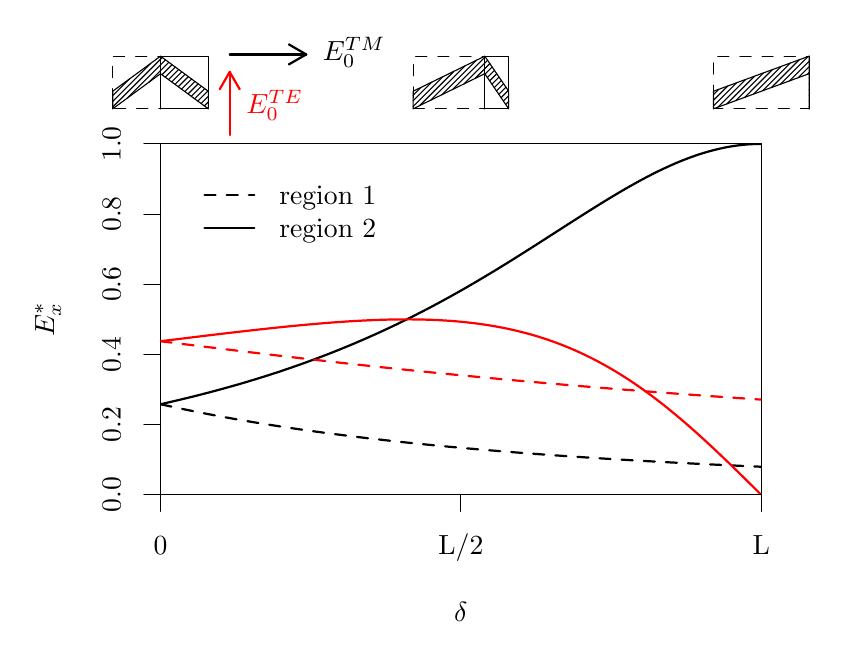
\begin{tikzpicture}[x=1pt,y=1pt]
\definecolor[named]{fillColor}{rgb}{1.00,1.00,1.00}
\path[use as bounding box,fill=fillColor,fill opacity=0.00] (0,0) rectangle (289.08,216.81);
\begin{scope}
\path[clip] ( 48.00, 48.00) rectangle (265.08,174.81);
\definecolor[named]{drawColor}{rgb}{0.00,0.00,0.00}

\path[draw=drawColor,line width= 0.8pt,dash pattern=on 4pt off 4pt ,line join=round,line cap=round] ( 48.00, 80.74) --
	( 50.19, 80.26) --
	( 52.39, 79.78) --
	( 54.58, 79.32) --
	( 56.77, 78.86) --
	( 58.96, 78.41) --
	( 61.16, 77.97) --
	( 63.35, 77.54) --
	( 65.54, 77.11) --
	( 67.73, 76.70) --
	( 69.93, 76.29) --
	( 72.12, 75.89) --
	( 74.31, 75.50) --
	( 76.51, 75.12) --
	( 78.70, 74.74) --
	( 80.89, 74.37) --
	( 83.08, 74.01) --
	( 85.28, 73.65) --
	( 87.47, 73.30) --
	( 89.66, 72.96) --
	( 91.85, 72.62) --
	( 94.05, 72.29) --
	( 96.24, 71.97) --
	( 98.43, 71.65) --
	(100.63, 71.33) --
	(102.82, 71.03) --
	(105.01, 70.73) --
	(107.20, 70.43) --
	(109.40, 70.14) --
	(111.59, 69.86) --
	(113.78, 69.58) --
	(115.97, 69.30) --
	(118.17, 69.03) --
	(120.36, 68.76) --
	(122.55, 68.50) --
	(124.75, 68.25) --
	(126.94, 68.00) --
	(129.13, 67.75) --
	(131.32, 67.51) --
	(133.52, 67.27) --
	(135.71, 67.03) --
	(137.90, 66.80) --
	(140.09, 66.57) --
	(142.29, 66.35) --
	(144.48, 66.13) --
	(146.67, 65.92) --
	(148.87, 65.70) --
	(151.06, 65.50) --
	(153.25, 65.29) --
	(155.44, 65.09) --
	(157.64, 64.89) --
	(159.83, 64.70) --
	(162.02, 64.51) --
	(164.21, 64.32) --
	(166.41, 64.13) --
	(168.60, 63.95) --
	(170.79, 63.77) --
	(172.99, 63.59) --
	(175.18, 63.42) --
	(177.37, 63.25) --
	(179.56, 63.08) --
	(181.76, 62.91) --
	(183.95, 62.75) --
	(186.14, 62.59) --
	(188.33, 62.43) --
	(190.53, 62.27) --
	(192.72, 62.12) --
	(194.91, 61.97) --
	(197.11, 61.82) --
	(199.30, 61.68) --
	(201.49, 61.53) --
	(203.68, 61.39) --
	(205.88, 61.25) --
	(208.07, 61.11) --
	(210.26, 60.98) --
	(212.45, 60.84) --
	(214.65, 60.71) --
	(216.84, 60.58) --
	(219.03, 60.45) --
	(221.23, 60.33) --
	(223.42, 60.20) --
	(225.61, 60.08) --
	(227.80, 59.96) --
	(230.00, 59.84) --
	(232.19, 59.72) --
	(234.38, 59.61) --
	(236.57, 59.50) --
	(238.77, 59.38) --
	(240.96, 59.27) --
	(243.15, 59.16) --
	(245.35, 59.06) --
	(247.54, 58.95) --
	(249.73, 58.85) --
	(251.92, 58.74) --
	(254.12, 58.64) --
	(256.31, 58.54) --
	(258.50, 58.44) --
	(260.69, 58.34) --
	(262.89, 58.25) --
	(265.08, 58.15);
\end{scope}
\begin{scope}
\path[clip] (  0.00,  0.00) rectangle (289.08,216.81);
\definecolor[named]{drawColor}{rgb}{0.00,0.00,0.00}

\path[draw=drawColor,line width= 0.4pt,line join=round,line cap=round] ( 48.00, 48.00) -- ( 48.00,174.81);

\path[draw=drawColor,line width= 0.4pt,line join=round,line cap=round] ( 48.00, 48.00) -- ( 42.00, 48.00);

\path[draw=drawColor,line width= 0.4pt,line join=round,line cap=round] ( 48.00, 73.36) -- ( 42.00, 73.36);

\path[draw=drawColor,line width= 0.4pt,line join=round,line cap=round] ( 48.00, 98.72) -- ( 42.00, 98.72);

\path[draw=drawColor,line width= 0.4pt,line join=round,line cap=round] ( 48.00,124.09) -- ( 42.00,124.09);

\path[draw=drawColor,line width= 0.4pt,line join=round,line cap=round] ( 48.00,149.45) -- ( 42.00,149.45);

\path[draw=drawColor,line width= 0.4pt,line join=round,line cap=round] ( 48.00,174.81) -- ( 42.00,174.81);

\node[text=drawColor,rotate= 90.00,anchor=base,inner sep=0pt, outer sep=0pt, scale=  1.00] at ( 33.60, 48.00) {0.0};

\node[text=drawColor,rotate= 90.00,anchor=base,inner sep=0pt, outer sep=0pt, scale=  1.00] at ( 33.60, 73.36) {0.2};

\node[text=drawColor,rotate= 90.00,anchor=base,inner sep=0pt, outer sep=0pt, scale=  1.00] at ( 33.60, 98.72) {0.4};

\node[text=drawColor,rotate= 90.00,anchor=base,inner sep=0pt, outer sep=0pt, scale=  1.00] at ( 33.60,124.09) {0.6};

\node[text=drawColor,rotate= 90.00,anchor=base,inner sep=0pt, outer sep=0pt, scale=  1.00] at ( 33.60,149.45) {0.8};

\node[text=drawColor,rotate= 90.00,anchor=base,inner sep=0pt, outer sep=0pt, scale=  1.00] at ( 33.60,174.81) {1.0};

\path[draw=drawColor,line width= 0.4pt,line join=round,line cap=round] ( 48.00, 48.00) --
	(265.08, 48.00) --
	(265.08,174.81) --
	( 48.00,174.81) --
	( 48.00, 48.00);
\end{scope}
\begin{scope}
\path[clip] (  0.00,  0.00) rectangle (289.08,216.81);
\definecolor[named]{drawColor}{rgb}{0.00,0.00,0.00}

\node[text=drawColor,anchor=base,inner sep=0pt, outer sep=0pt, scale=  1.00] at (156.54,  2.40) {$\delta$};

\node[text=drawColor,rotate= 90.00,anchor=base,inner sep=0pt, outer sep=0pt, scale=  1.00] at (  9.60,111.41) {$E_x^*$};
\end{scope}
\begin{scope}
\path[clip] ( 48.00, 48.00) rectangle (265.08,174.81);
\definecolor[named]{drawColor}{rgb}{0.00,0.00,0.00}

\path[draw=drawColor,line width= 0.8pt,line join=round,line cap=round] ( 48.00, 80.74) --
	( 50.19, 81.24) --
	( 52.39, 81.75) --
	( 54.58, 82.26) --
	( 56.77, 82.79) --
	( 58.96, 83.32) --
	( 61.16, 83.87) --
	( 63.35, 84.43) --
	( 65.54, 85.00) --
	( 67.73, 85.58) --
	( 69.93, 86.18) --
	( 72.12, 86.78) --
	( 74.31, 87.40) --
	( 76.51, 88.03) --
	( 78.70, 88.67) --
	( 80.89, 89.33) --
	( 83.08, 90.00) --
	( 85.28, 90.68) --
	( 87.47, 91.38) --
	( 89.66, 92.09) --
	( 91.85, 92.82) --
	( 94.05, 93.56) --
	( 96.24, 94.32) --
	( 98.43, 95.09) --
	(100.63, 95.88) --
	(102.82, 96.68) --
	(105.01, 97.50) --
	(107.20, 98.33) --
	(109.40, 99.18) --
	(111.59,100.05) --
	(113.78,100.94) --
	(115.97,101.84) --
	(118.17,102.76) --
	(120.36,103.70) --
	(122.55,104.65) --
	(124.75,105.63) --
	(126.94,106.62) --
	(129.13,107.63) --
	(131.32,108.66) --
	(133.52,109.70) --
	(135.71,110.77) --
	(137.90,111.85) --
	(140.09,112.95) --
	(142.29,114.08) --
	(144.48,115.21) --
	(146.67,116.37) --
	(148.87,117.55) --
	(151.06,118.74) --
	(153.25,119.95) --
	(155.44,121.18) --
	(157.64,122.43) --
	(159.83,123.69) --
	(162.02,124.97) --
	(164.21,126.27) --
	(166.41,127.58) --
	(168.60,128.90) --
	(170.79,130.24) --
	(172.99,131.59) --
	(175.18,132.95) --
	(177.37,134.33) --
	(179.56,135.71) --
	(181.76,137.10) --
	(183.95,138.50) --
	(186.14,139.90) --
	(188.33,141.31) --
	(190.53,142.72) --
	(192.72,144.13) --
	(194.91,145.54) --
	(197.11,146.94) --
	(199.30,148.34) --
	(201.49,149.73) --
	(203.68,151.11) --
	(205.88,152.48) --
	(208.07,153.84) --
	(210.26,155.18) --
	(212.45,156.49) --
	(214.65,157.79) --
	(216.84,159.06) --
	(219.03,160.29) --
	(221.23,161.50) --
	(223.42,162.68) --
	(225.61,163.81) --
	(227.80,164.91) --
	(230.00,165.96) --
	(232.19,166.96) --
	(234.38,167.92) --
	(236.57,168.82) --
	(238.77,169.67) --
	(240.96,170.47) --
	(243.15,171.20) --
	(245.35,171.87) --
	(247.54,172.47) --
	(249.73,173.01) --
	(251.92,173.49) --
	(254.12,173.89) --
	(256.31,174.22) --
	(258.50,174.48) --
	(260.69,174.66) --
	(262.89,174.77) --
	(265.08,174.81);
\definecolor[named]{drawColor}{rgb}{1.00,0.00,0.00}

\path[draw=drawColor,line width= 0.8pt,dash pattern=on 4pt off 4pt ,line join=round,line cap=round] ( 48.00,103.50) --
	( 50.19,103.23) --
	( 52.39,102.96) --
	( 54.58,102.68) --
	( 56.77,102.41) --
	( 58.96,102.14) --
	( 61.16,101.87) --
	( 63.35,101.60) --
	( 65.54,101.33) --
	( 67.73,101.06) --
	( 69.93,100.79) --
	( 72.12,100.53) --
	( 74.31,100.26) --
	( 76.51, 99.99) --
	( 78.70, 99.73) --
	( 80.89, 99.46) --
	( 83.08, 99.20) --
	( 85.28, 98.94) --
	( 87.47, 98.68) --
	( 89.66, 98.42) --
	( 91.85, 98.16) --
	( 94.05, 97.90) --
	( 96.24, 97.65) --
	( 98.43, 97.39) --
	(100.63, 97.14) --
	(102.82, 96.89) --
	(105.01, 96.64) --
	(107.20, 96.39) --
	(109.40, 96.14) --
	(111.59, 95.89) --
	(113.78, 95.65) --
	(115.97, 95.41) --
	(118.17, 95.17) --
	(120.36, 94.93) --
	(122.55, 94.69) --
	(124.75, 94.45) --
	(126.94, 94.21) --
	(129.13, 93.98) --
	(131.32, 93.75) --
	(133.52, 93.52) --
	(135.71, 93.29) --
	(137.90, 93.06) --
	(140.09, 92.84) --
	(142.29, 92.61) --
	(144.48, 92.39) --
	(146.67, 92.17) --
	(148.87, 91.95) --
	(151.06, 91.73) --
	(153.25, 91.52) --
	(155.44, 91.30) --
	(157.64, 91.09) --
	(159.83, 90.88) --
	(162.02, 90.67) --
	(164.21, 90.46) --
	(166.41, 90.25) --
	(168.60, 90.05) --
	(170.79, 89.84) --
	(172.99, 89.64) --
	(175.18, 89.44) --
	(177.37, 89.24) --
	(179.56, 89.05) --
	(181.76, 88.85) --
	(183.95, 88.66) --
	(186.14, 88.46) --
	(188.33, 88.27) --
	(190.53, 88.08) --
	(192.72, 87.89) --
	(194.91, 87.70) --
	(197.11, 87.52) --
	(199.30, 87.33) --
	(201.49, 87.15) --
	(203.68, 86.97) --
	(205.88, 86.79) --
	(208.07, 86.61) --
	(210.26, 86.43) --
	(212.45, 86.26) --
	(214.65, 86.08) --
	(216.84, 85.91) --
	(219.03, 85.74) --
	(221.23, 85.57) --
	(223.42, 85.40) --
	(225.61, 85.23) --
	(227.80, 85.06) --
	(230.00, 84.90) --
	(232.19, 84.73) --
	(234.38, 84.57) --
	(236.57, 84.41) --
	(238.77, 84.25) --
	(240.96, 84.09) --
	(243.15, 83.93) --
	(245.35, 83.77) --
	(247.54, 83.62) --
	(249.73, 83.46) --
	(251.92, 83.31) --
	(254.12, 83.16) --
	(256.31, 83.01) --
	(258.50, 82.86) --
	(260.69, 82.71) --
	(262.89, 82.56) --
	(265.08, 82.41);

\path[draw=drawColor,line width= 0.8pt,line join=round,line cap=round] ( 48.00,103.50) --
	( 50.19,103.77) --
	( 52.39,104.04) --
	( 54.58,104.31) --
	( 56.77,104.58) --
	( 58.96,104.85) --
	( 61.16,105.11) --
	( 63.35,105.38) --
	( 65.54,105.65) --
	( 67.73,105.91) --
	( 69.93,106.17) --
	( 72.12,106.43) --
	( 74.31,106.69) --
	( 76.51,106.94) --
	( 78.70,107.19) --
	( 80.89,107.44) --
	( 83.08,107.68) --
	( 85.28,107.92) --
	( 87.47,108.16) --
	( 89.66,108.39) --
	( 91.85,108.62) --
	( 94.05,108.84) --
	( 96.24,109.06) --
	( 98.43,109.27) --
	(100.63,109.47) --
	(102.82,109.67) --
	(105.01,109.86) --
	(107.20,110.04) --
	(109.40,110.22) --
	(111.59,110.38) --
	(113.78,110.53) --
	(115.97,110.68) --
	(118.17,110.81) --
	(120.36,110.93) --
	(122.55,111.04) --
	(124.75,111.14) --
	(126.94,111.22) --
	(129.13,111.29) --
	(131.32,111.35) --
	(133.52,111.38) --
	(135.71,111.40) --
	(137.90,111.40) --
	(140.09,111.39) --
	(142.29,111.35) --
	(144.48,111.29) --
	(146.67,111.21) --
	(148.87,111.11) --
	(151.06,110.98) --
	(153.25,110.83) --
	(155.44,110.65) --
	(157.64,110.44) --
	(159.83,110.20) --
	(162.02,109.94) --
	(164.21,109.64) --
	(166.41,109.31) --
	(168.60,108.94) --
	(170.79,108.54) --
	(172.99,108.11) --
	(175.18,107.63) --
	(177.37,107.12) --
	(179.56,106.56) --
	(181.76,105.97) --
	(183.95,105.33) --
	(186.14,104.64) --
	(188.33,103.91) --
	(190.53,103.13) --
	(192.72,102.31) --
	(194.91,101.43) --
	(197.11,100.51) --
	(199.30, 99.54) --
	(201.49, 98.51) --
	(203.68, 97.43) --
	(205.88, 96.30) --
	(208.07, 95.11) --
	(210.26, 93.87) --
	(212.45, 92.58) --
	(214.65, 91.23) --
	(216.84, 89.83) --
	(219.03, 88.37) --
	(221.23, 86.86) --
	(223.42, 85.30) --
	(225.61, 83.69) --
	(227.80, 82.03) --
	(230.00, 80.31) --
	(232.19, 78.55) --
	(234.38, 76.74) --
	(236.57, 74.89) --
	(238.77, 73.00) --
	(240.96, 71.06) --
	(243.15, 69.09) --
	(245.35, 67.09) --
	(247.54, 65.05) --
	(249.73, 62.98) --
	(251.92, 60.89) --
	(254.12, 58.78) --
	(256.31, 56.64) --
	(258.50, 54.50) --
	(260.69, 52.34) --
	(262.89, 50.17) --
	(265.08, 48.00);
\end{scope}
\begin{scope}
\path[clip] (  0.00,  0.00) rectangle (289.08,216.81);
\definecolor[named]{drawColor}{rgb}{0.00,0.00,0.00}

\path[draw=drawColor,line width= 0.4pt,line join=round,line cap=round] ( 48.00, 48.00) -- (265.08, 48.00);

\path[draw=drawColor,line width= 0.4pt,line join=round,line cap=round] ( 48.00, 48.00) -- ( 48.00, 42.00);

\path[draw=drawColor,line width= 0.4pt,line join=round,line cap=round] (156.54, 48.00) -- (156.54, 42.00);

\path[draw=drawColor,line width= 0.4pt,line join=round,line cap=round] (265.08, 48.00) -- (265.08, 42.00);

\node[text=drawColor,anchor=base,inner sep=0pt, outer sep=0pt, scale=  1.00] at ( 48.00, 26.40) {0};

\node[text=drawColor,anchor=base,inner sep=0pt, outer sep=0pt, scale=  1.00] at (156.54, 26.40) {L/2};

\node[text=drawColor,anchor=base,inner sep=0pt, outer sep=0pt, scale=  1.00] at (265.08, 26.40) {L};
\end{scope}
\begin{scope}
\path[clip] (  0.00,  0.00) rectangle (289.08,216.81);
\definecolor[named]{drawColor}{rgb}{0.00,0.00,0.00}

\path[draw=drawColor,line width= 0.4pt,line join=round,line cap=round] ( 30.73,192.21) -- ( 36.82,198.31);

\path[draw=drawColor,line width= 0.4pt,line join=round,line cap=round] ( 30.73,190.17) -- ( 44.51,203.95);

\path[draw=drawColor,line width= 0.4pt,line join=round,line cap=round] ( 30.73,188.12) -- ( 48.64,206.04);

\path[draw=drawColor,line width= 0.4pt,line join=round,line cap=round] ( 36.04,191.39) -- ( 49.82,205.17);

\path[draw=drawColor,line width= 0.4pt,line join=round,line cap=round] ( 43.73,197.04) -- ( 51.00,204.31);

\path[draw=drawColor,line width= 0.4pt,line join=round,line cap=round] ( 48.52,199.79) -- ( 52.18,203.44);

\path[draw=drawColor,line width= 0.4pt,line join=round,line cap=round] ( 49.70,198.92) -- ( 53.36,202.58);

\path[draw=drawColor,line width= 0.4pt,line join=round,line cap=round] ( 50.88,198.06) -- ( 54.54,201.71);

\path[draw=drawColor,line width= 0.4pt,line join=round,line cap=round] ( 52.06,197.19) -- ( 55.72,200.85);

\path[draw=drawColor,line width= 0.4pt,line join=round,line cap=round] ( 53.24,196.33) -- ( 56.90,199.98);

\path[draw=drawColor,line width= 0.4pt,line join=round,line cap=round] ( 54.42,195.46) -- ( 58.07,199.12);

\path[draw=drawColor,line width= 0.4pt,line join=round,line cap=round] ( 55.60,194.60) -- ( 59.25,198.25);

\path[draw=drawColor,line width= 0.4pt,line join=round,line cap=round] ( 56.78,193.73) -- ( 60.43,197.39);

\path[draw=drawColor,line width= 0.4pt,line join=round,line cap=round] ( 57.95,192.86) -- ( 61.61,196.52);

\path[draw=drawColor,line width= 0.4pt,line join=round,line cap=round] ( 59.13,192.00) -- ( 62.79,195.66);

\path[draw=drawColor,line width= 0.4pt,line join=round,line cap=round] ( 60.31,191.13) -- ( 63.97,194.79);

\path[draw=drawColor,line width= 0.4pt,line join=round,line cap=round] ( 61.49,190.27) -- ( 65.15,193.93);

\path[draw=drawColor,line width= 0.4pt,line join=round,line cap=round] ( 62.67,189.40) -- ( 65.27,192.01);

\path[draw=drawColor,line width= 0.4pt,line join=round,line cap=round] ( 63.85,188.54) -- ( 65.27,189.97);

\path[draw=drawColor,line width= 0.4pt,line join=round,line cap=round] ( 65.03,187.67) -- ( 65.27,187.92);

\path[draw=drawColor,line width= 0.4pt,line join=round,line cap=round] ( 30.73,193.83) --
	( 48.00,206.51) --
	( 65.27,193.83) --
	( 65.27,187.49) --
	( 48.00,200.17) --
	( 30.73,187.49) --
	( 30.73,193.83);

\path[draw=drawColor,line width= 0.4pt,line join=round,line cap=round] ( 48.00,187.49) --
	( 48.00,206.51) --
	( 65.27,206.51) --
	( 65.27,187.49) --
	( 48.00,187.49);

\path[draw=drawColor,line width= 0.4pt,dash pattern=on 4pt off 4pt ,line join=round,line cap=round] ( 48.00,187.49) --
	( 48.00,206.51) --
	( 30.73,206.51) --
	( 30.73,187.49) --
	( 48.00,187.49);

\path[draw=drawColor,line width= 0.4pt,line join=round,line cap=round] (247.81,192.61) -- (249.73,194.54);

\path[draw=drawColor,line width= 0.4pt,line join=round,line cap=round] (247.81,190.57) -- (252.96,195.72);

\path[draw=drawColor,line width= 0.4pt,line join=round,line cap=round] (247.81,188.53) -- (256.19,196.91);

\path[draw=drawColor,line width= 0.4pt,line join=round,line cap=round] (249.40,188.08) -- (259.42,198.09);

\path[draw=drawColor,line width= 0.4pt,line join=round,line cap=round] (252.63,189.26) -- (262.65,199.28);

\path[draw=drawColor,line width= 0.4pt,line join=round,line cap=round] (255.86,190.45) -- (265.88,200.46);

\path[draw=drawColor,line width= 0.4pt,line join=round,line cap=round] (259.09,191.63) -- (269.10,201.65);

\path[draw=drawColor,line width= 0.4pt,line join=round,line cap=round] (262.32,192.82) -- (272.33,202.83);

\path[draw=drawColor,line width= 0.4pt,line join=round,line cap=round] (265.55,194.00) -- (275.56,204.02);

\path[draw=drawColor,line width= 0.4pt,line join=round,line cap=round] (268.78,195.19) -- (278.79,205.21);

\path[draw=drawColor,line width= 0.4pt,line join=round,line cap=round] (272.01,196.37) -- (282.02,206.39);

\path[draw=drawColor,line width= 0.4pt,line join=round,line cap=round] (275.23,197.56) -- (282.35,204.68);

\path[draw=drawColor,line width= 0.4pt,line join=round,line cap=round] (278.46,198.74) -- (282.35,202.63);

\path[draw=drawColor,line width= 0.4pt,line join=round,line cap=round] (281.69,199.93) -- (282.35,200.59);

\path[draw=drawColor,line width= 0.4pt,line join=round,line cap=round] (282.35,198.55) -- (282.35,198.55);

\path[draw=drawColor,line width= 0.4pt,line join=round,line cap=round] (282.35,196.50) -- (282.35,196.50);

\path[draw=drawColor,line width= 0.4pt,line join=round,line cap=round] (282.35,194.46) -- (282.35,194.46);

\path[draw=drawColor,line width= 0.4pt,line join=round,line cap=round] (282.35,192.41) -- (282.35,192.41);

\path[draw=drawColor,line width= 0.4pt,line join=round,line cap=round] (282.35,190.37) -- (282.35,190.37);

\path[draw=drawColor,line width= 0.4pt,line join=round,line cap=round] (282.35,188.33) -- (282.35,188.33);

\path[draw=drawColor,line width= 0.4pt,line join=round,line cap=round] (247.81,193.83) --
	(282.35,206.51) --
	(282.35,193.83) --
	(282.35,187.49) --
	(282.35,200.17) --
	(247.81,187.49) --
	(247.81,193.83);

\path[draw=drawColor,line width= 0.4pt,line join=round,line cap=round] (282.35,187.49) --
	(282.35,206.51) --
	(282.35,206.51) --
	(282.35,187.49) --
	(282.35,187.49);

\path[draw=drawColor,line width= 0.4pt,dash pattern=on 4pt off 4pt ,line join=round,line cap=round] (282.35,187.49) --
	(282.35,206.51) --
	(247.81,206.51) --
	(247.81,187.49) --
	(282.35,187.49);

\path[draw=drawColor,line width= 0.4pt,line join=round,line cap=round] (139.27,192.41) -- (142.05,195.19);

\path[draw=drawColor,line width= 0.4pt,line join=round,line cap=round] (139.27,190.37) -- (146.05,197.15);

\path[draw=drawColor,line width= 0.4pt,line join=round,line cap=round] (139.27,188.32) -- (150.05,199.11);

\path[draw=drawColor,line width= 0.4pt,line join=round,line cap=round] (141.64,188.65) -- (154.05,201.07);

\path[draw=drawColor,line width= 0.4pt,line join=round,line cap=round] (145.64,190.61) -- (158.06,203.03);

\path[draw=drawColor,line width= 0.4pt,line join=round,line cap=round] (149.64,192.57) -- (162.06,204.99);

\path[draw=drawColor,line width= 0.4pt,line join=round,line cap=round] (153.65,194.53) -- (165.36,206.24);

\path[draw=drawColor,line width= 0.4pt,line join=round,line cap=round] (157.65,196.49) -- (166.19,205.03);

\path[draw=drawColor,line width= 0.4pt,line join=round,line cap=round] (161.65,198.45) -- (167.02,203.81);

\path[draw=drawColor,line width= 0.4pt,line join=round,line cap=round] (165.28,200.03) -- (167.85,202.60);

\path[draw=drawColor,line width= 0.4pt,line join=round,line cap=round] (166.10,198.81) -- (168.67,201.38);

\path[draw=drawColor,line width= 0.4pt,line join=round,line cap=round] (166.93,197.59) -- (169.50,200.16);

\path[draw=drawColor,line width= 0.4pt,line join=round,line cap=round] (167.76,196.38) -- (170.33,198.95);

\path[draw=drawColor,line width= 0.4pt,line join=round,line cap=round] (168.59,195.16) -- (171.16,197.73);

\path[draw=drawColor,line width= 0.4pt,line join=round,line cap=round] (169.42,193.95) -- (171.99,196.52);

\path[draw=drawColor,line width= 0.4pt,line join=round,line cap=round] (170.25,192.73) -- (172.81,195.30);

\path[draw=drawColor,line width= 0.4pt,line join=round,line cap=round] (171.07,191.51) -- (173.64,194.08);

\path[draw=drawColor,line width= 0.4pt,line join=round,line cap=round] (171.90,190.30) -- (173.81,192.21);

\path[draw=drawColor,line width= 0.4pt,line join=round,line cap=round] (172.73,189.08) -- (173.81,190.17);

\path[draw=drawColor,line width= 0.4pt,line join=round,line cap=round] (173.56,187.87) -- (173.81,188.12);

\path[draw=drawColor,line width= 0.4pt,line join=round,line cap=round] (139.27,193.83) --
	(165.18,206.51) --
	(173.81,193.83) --
	(173.81,187.49) --
	(165.18,200.17) --
	(139.27,187.49) --
	(139.27,193.83);

\path[draw=drawColor,line width= 0.4pt,line join=round,line cap=round] (165.18,187.49) --
	(165.18,206.51) --
	(173.81,206.51) --
	(173.81,187.49) --
	(165.18,187.49);

\path[draw=drawColor,line width= 0.4pt,dash pattern=on 4pt off 4pt ,line join=round,line cap=round] (165.18,187.49) --
	(165.18,206.51) --
	(139.27,206.51) --
	(139.27,187.49) --
	(165.18,187.49);

\path[draw=drawColor,line width= 0.8pt,line join=round,line cap=round] ( 73.00,207.15) -- (100.64,207.15);

\path[draw=drawColor,line width= 0.8pt,line join=round,line cap=round] ( 94.38,203.53) --
	(100.64,207.15) --
	( 94.38,210.76);

\node[text=drawColor,anchor=base west,inner sep=0pt, outer sep=0pt, scale=  1.00] at (106.64,204.85) {$E_0^{TM}$};
\definecolor[named]{drawColor}{rgb}{1.00,0.00,0.00}

\path[draw=drawColor,line width= 0.8pt,line join=round,line cap=round] ( 73.00,177.98) -- ( 73.00,200.81);

\path[draw=drawColor,line width= 0.8pt,line join=round,line cap=round] ( 76.61,194.55) --
	( 73.00,200.81) --
	( 69.39,194.55);

\node[text=drawColor,anchor=base west,inner sep=0pt, outer sep=0pt, scale=  1.00] at ( 79.00,185.83) {$E_0^{TE}$};

\path[] ( 54.91,168.47) rectangle (130.43,132.47);
\definecolor[named]{drawColor}{rgb}{0.00,0.00,0.00}

\path[draw=drawColor,line width= 0.8pt,dash pattern=on 4pt off 4pt ,line join=round,line cap=round] ( 63.91,156.47) -- ( 81.91,156.47);

\path[draw=drawColor,line width= 0.8pt,line join=round,line cap=round] ( 63.91,144.47) -- ( 81.91,144.47);

\node[text=drawColor,anchor=base west,inner sep=0pt, outer sep=0pt, scale=  1.00] at ( 90.91,153.03) {region 1};

\node[text=drawColor,anchor=base west,inner sep=0pt, outer sep=0pt, scale=  1.00] at ( 90.91,141.03) {region 2};
\end{scope}
\end{tikzpicture}
